\documentclass{article}


\usepackage[utf8]{inputenc}
\usepackage[T1]{fontenc}
\usepackage[brazil]{babel}
\usepackage[pdftex,pagebackref=true,colorlinks=true,linkcolor=blue,unicode]{hyperref}
\usepackage[paper=a4paper,lmargin=2.0cm, rmargin=2.0cm, tmargin=2.0cm, bmargin=2.0cm]{geometry}
\usepackage{graphicx}
\usepackage{makeidx}
\usepackage{hyperref}
\usepackage{enumerate}
\usepackage{indentfirst}
\usepackage{algorithm2e}
\usepackage{algorithmic}

%\renewcommand{algorithm}{Algoritmo}
%\renewcommand{\listalgorithmname}{Lista de Algoritmos}

\title{Grafo Clique e Grafo Cordal}
\author{Roberto Beraldo Chaiben}
%\date{}


\makeindex


\begin{document}


\maketitle
\tableofcontents
\listofalgorithms


\newpage


%====================================================

\section{Grafo Clique}

Consideremos um \index{grafo}grafo $G$. O \index{grafo clique}grafo clique de
$G$, denotado por $K(G)$, tem como \index{vértices}vértices as
\index{cliques}cliques maximais de $G$, e dois vértices de $K(G)$ são adjacentes
se as respectivas cliques de $G$ tem \index{intersecção}intersecção.


Grafos clique constituem uma classe especial de grafos de intersecção, sobre
os quais se interessam aspectos relativos à caracterização, determinação do
\index{número de estabilidade}número de estabilidade e do
\index{número cromático}número cromático (problemas ainda não resolvidos de
forma satisfatória para esta classe de grafos).


\begin{figure}[h]
    \center
    \caption{Grafo $G$: Grafo com quatro cliques maximais}
    \label{fig:1}
    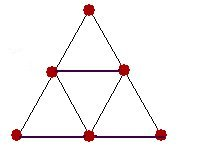
\includegraphics[width=3cm]{img/clique01.jpg}
\end{figure}

\begin{figure}[h]
    \center
    \caption{Grafo $K(G)$: Grafo clique do grafo da figura 1}
    \label{fig:2}
    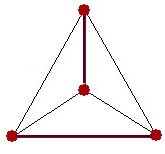
\includegraphics[width=3cm]{img/clique02.jpg}
\end{figure}

A Figura \ref{fig:1} mostra um grafo $G$ com quatro
\index{cliques maximais}cliques maximais, as quais tornam-se
\index{vértices}vértices de seu \index{grafo clique}grafo clique $K(G)$, o qual
está ilustrado na Figura \ref{fig:2}.


\subsection{Algoritmo de Bron-Kerbosch}

O \index{algoritmo}algoritmo de \index{Bron-Kerbosch}Bron-Kerbosch é utilizado
para encontrar as cliques maximais de um grafo $G$. O algoritmo utiliza um
\index{backtracking}\textit{backtracking} \index{recursivo} para encontrar
todas as cliques maximais do grafo $G$.

Mais genericamente, dados três conjuntos $R$, $P$ e $X$, o algoritmo encontra
as cliques maximais que incluem todos os vértices em $R$, alguns dos vértices
em $P$, e nenhum dos vértices em $X$. Nas chamadas recursivas do algoritmo, $P$
e $X$ são restritos aos vértices que formam adicionados a $R$, uma vez que
estes são os vértices que só podem ser usados como parte da saída ou para
evitar alguma clique de ser considerada como saída.


A \index{recursão}recursão é iniciada através da definição de $R$ e $X$ como
conjuntos vazios e $P$ o vértice definido do grafo. A cada chamada recursiva,
o \index{algoritmo}algoritmo considera os vértices de $P$ corrente, se não há
vértices em $P$, considera $R$ como uma clique maximal (se X é vazio), ou faz
\index{backtracking}\textit{backtracking}. Para cada vértice $v$ de $P$, ele
faz uma chamada recursiva em que $v$ é adicionado a $R$, em que $P$ e $X$ são
restritas aos vizinhos de $v$, $N(v)$, que localiza e considera todas as
extensões de $R$ que contêm $v$. Então, ele move $v$ de $P$ para $X$ e continua
com o próximo vértice em $P$.



\begin{algorithm}
    \KwData{ Conjuntos P, R e X }
    \KwResult{ Cliques maximais do grafo G }
    \caption{Algoritmo de Bron-Kerbosch}
    \label{alg:bronkerbosch}
    
    \begin{algorithmic}
    
    \IF{ P e X são vazios}
        \STATE{considera R como clique maximal}
    \ENDIF
    
    \FOR{ \textbf{each} vértice $v$ em $P$ }
           \STATE{Bron-Kerbosch1($R \cup {v}, P \cap N(v), X \cap N(v))$}
           \STATE{$P := P \backslash \{v\}$}
           \STATE{$X := X \cup {v}$}
     \ENDFOR
    
    \end{algorithmic}
\end{algorithm}




\section{Grafos Cordais}

\index{grafos cordais}Grafos cordais são grafos em que todo
\index{circuito}circuito de 4 ou mais vértices desse grafo possui uma
\index{corda}corda, ou seja, uma \index{aresta}aresta não pertencente ao
\index{ciclo}ciclo ligando dois vértices não \index{adjacentes}adjacentes no
\index{circuito}circuito.

\begin{figure}[h]
    \center
    \caption{Grafo cordal}
    \label{fig:cordal}
    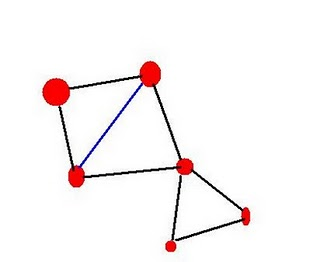
\includegraphics[width=7cm]{img/cordal01.jpg}
\end{figure}


A Figura \ref{fig:cordal} é um exemplo de grafo cordal.\\


Em \index{grafos cordais}grafos cordais, alguns problemas que seriam
\index{NP-difícil}NP-difíceis em grafos genéricos tornam-se passíveis de
resolução em tempo polinomial. Entre esses problemas, temos o problema de
encontrar o \index{clique máximo}clique máximo, o maior
\index{conjunto independente}conjunto independente, entre outros.


\subsection{ Algoritmo de Busca em Largura Lexicográfica - Lex-BFS }


A detecção de grafos cordais pode ser feita em tempo O(n+m) por meio de uma
importante ferramenta que será útil na resolução de outros problemas como o
de encontrar o clique máximo no grafo. Essa ferramenta é o
\index{Lex-BFS}Lex-BFS, ou
\index{Busca em Largura Lexicográfica}Busca em Largura Lexicográfica, um
algoritmo que gera uma \index{ordenação}ordenação dos vértices com propriedades
importantes para a resolução de diversos problemas em grafos.




\begin{algorithm}
    \KwData{ Um grafo não-dirigido $G$, com o conjunto de vértices $V$ e com o conjunto de arestas $E$. }
    \KwResult{ Uma ordenação dos vértices de $G$ }
    \caption{Busca em Largura Lexicográfica}
    \label{alg:lexbfs}
    
    \begin{algorithmic}

        \STATE $L$ = $(V)$ \COMMENT{$L$ é uma família ordenada de conjuntos que recebe inicialmente o conjunto dos vítices $V$ em qualquer ordem }\;
        \STATE $i$ = $n - 1$\;
        
        \WHILE{ $L$ não está vazia}
            \STATE $S$ = $L$.front() \COMMENT{$S$ é o primeiro conjunto de $L$}\;
            \STATE $x$ = $S$.front()  \COMMENT{$x$ é o primeiro elemento de $S$}\;
            \STATE $S$.pop\_front()  \COMMENT{retire $x$ de $S$}\;
                  
            \IF{ $S$ ficou vazio}
                \STATE{ $L$.pop\_front() }
            \ENDIF
                  
            \STATE $pi$[x] = i \;
            \STATE $i--$ \;
             
             \FOR{ cada conjunto $S$ em $L$ }
                \STATE $Y$ = \{elementos em $S$ que são adjacentes a $x$\}\;
                \IF{ $Y$ for não vazio e diferente de $S$ }
                    \STATE{ insira $Y$ antes de $S$ em $L$ e retire $Y$ de $S$}
                \ENDIF
             \ENDFOR
         \ENDWHILE
        
         \RETURN $pi$

    \end{algorithmic}
\end{algorithm}




O \index{Lex-BFS}Lex-BFS executa $n$ vezes o \index{loop}loop sobre os
conjuntos existentes em $L$ e particiona cada conjunto de $L$ em duas partes:
a dos adjacentes a $x$ e a dos não adjacentes. Essas operações podem ser
executadas proporcionalmente ao numero de adjacentes a $x$. Como cada $x$ é
pivô somente uma vez, cada aresta será visitada somente uma vez, logo a
complexidade do Lex-BFS fica em $O(n+m)$.


O vetor $pi$ retornado pelo Lex-BFS indica a ordem de cada vértice $x$ na
sequência de visitas efetuada pelo algoritmo. Com base nesse vetor, definiremos
um outro conjunto associado a cada vértice do grafo $G$. Esse conjunto é o
$RN(x)$, o conjunto dos vértices adjacentes a $x$ que estão a direita de $x$
na ordem voltada pelo Lex-BFS:

\begin{equation}
    RN(x) = \{ y \  adjacente a \  x: pi[y] > pi[x] \}
\end{equation}

Um elemento importante em $RN(x)$ é o $parent(x)$, que é o elemento mais a
esquerda em $RN(x)$, ou seja, o elemento $y$ em $RN(x)$ com menor $pi[y]$.

O algoritmo de detecção de grafos cordais usa o seguinte resultado para
verificar se um grafo é cordal:

\begin{quotation}
"Um grafo é cordal se, e somente se, a ordenação de vértices voltada pelo
Lex-BFS é um \index{esquema de eliminação perfeito}esquema de eliminação perfeito."
\end{quotation}

Um esquema de \index{esquema de eliminação perfeito}eliminação perfeito é uma
ordenação de vértices $V[0],V[1], ... , V[n-1]$ de tal forma que para todo
vértice $V[j]$ anterior e adjacente a $V[i]$, o conjunto dos adjacentes de
$V[j]$ está contido no conjunto dos adjacentes de $V[i]$. O algoritmo de teste
de cordalidade basicamente é isso, verifica se os adjucantes a direita de cada
vértice $x$ está contido no conjunto dos adjacentes a direita de $parent(x)$.


\begin{algorithm}
    \KwData{ Um grafo não-dirigido $G$, com o conjunto de vértices $V$ e com o conjunto de arestas $E$. }
    \KwResult{ $TRUE$ se o grafo é cordal, $FALSE$ caso contrário }
    \caption{isChordal}
    \label{alg:ischordal}
    
    \begin{algorithmic}
    
        \STATE $pi$ = Lex\_BFS(G)\;
        \STATE $RN$ = \{$RN(x)$ de cada vértice de $G$\}\;
        \STATE $parent$ = \{$parent(x)$ de cada vértice de $G$, ou seja, o elemento $y$ em $RN(x)$ com menor $pi(y)$\}\;
       
        \FOR{ cada vértice $x$ em $G$}
            \IF{ \{$RN(x) - \{parent(x)$ \} \} não está contido em $RN(parent(x)$}       
                \RETURN FALSE\;
            \ENDIF
       \ENDFOR
       
       \RETURN TRUE
    
    \end{algorithmic}
\end{algorithm}



Como a construção de $RN(x)$ pode ser feita em $O(m)$ e a verificação de que
$RN(x)-parent(x)$ está contida em $RN(parent(x))$ pode ser feita em $O(1)$, a
complexidade do algoritmo fica em $O(m+n)$.





%====================================



\printindex



\end{document}
